\documentclass[lettersize,journal]{IEEEtran}
\usepackage{amsmath,amsfonts}
\usepackage{algorithmic}
\usepackage{array}
\usepackage[caption=false,font=normalsize,labelfont=sf,textfont=sf]{subfig}
\usepackage{textcomp}
\usepackage{stfloats}
\usepackage{url}
\usepackage{verbatim}
\usepackage{graphicx}
\usepackage{svg}
\usepackage{subfigure}
\usepackage{subcaption}
\hyphenation{op-tical net-works semi-conduc-tor IEEE-Xplore}
\def\BibTeX{{\rm B\kern-.05em{\sc i\kern-.025em b}\kern-.08em
    T\kern-.1667em\lower.7ex\hbox{E}\kern-.125emX}}
\usepackage{balance}
\begin{document}
\title{How to Use the IEEEtran \LaTeX \ Templates}
\author{IEEE Publication Technology Department}

\markboth{Journal of \LaTeX\ Class Files,~Vol.~18, No.~9, September~2020}%
{How to Use the IEEEtran \LaTeX \ Templates}

\maketitle

\begin{abstract}

\end{abstract}

\begin{IEEEkeywords}

\end{IEEEkeywords}


\section{Introduction}
\IEEEPARstart{A}{s} High Performance Computing workloads continue to grow into the exascale realm, and as hardware scales to match it, some old challenges become ever more important to resolve. One of said challenges is the appearance of radiation induced bit flips inside computational units. Sometimes, either due to cosmic rays or passive radiation from packaging materials, a bit inside the state of a chip can flip and then end up as a noticeable change in the architectural state of the execution.\cite{dodd2003basic,doi:10.1126/science.206.4420.776} The scale of modern HPC systems increases the likelihood of these events to a point at which they need to be dealt with in a proactive manner.\cite{geist2016supercomputing,snir2014addressing,dongarra2015fault} \\
The impact on the execution state is normally separated in three major categories:\cite{avizienis2004basic}
\begin{itemize}
    \item None: The fault did not result in a noticeable change in
the execution state and the program finished as if no fault
had occurred.
\item Crash: The fault generated a change in the state that at
some further point in execution resulted in a segmentation
fault.
\item Silent Data Corruption: The fault resulted in a change to
the architectural state that allowed the program to finish
successfully but with a visible difference in the output
returned
\end{itemize}

In this paper we will focus on SDCs. While crashes can be expensive to recover from, they are always caught. SDCs introduce a constant doubt upon the results obtained, and considering many HPC applications are in the scientific domain (where high precision is required and where an easy method to check results is not always available) confidence in the outputs is paramount.\\
Most fault tolerance in HPC executions is done through software methods like checkpoint-recovery. \cite{snir2014addressing}These methods are increasingly sensitive to the ever growing scale of HPC applications. Therefore, there has been a substantial push to protection methods at the hardware level in order to mitigate the increasing cost of check pointing.  \\
The ephemeral nature of transient faults presents a significant challenge in designing protection methods at the hardware level to shield against them. Since they only exist during the execution of an instruction, the only way to catch a fault is by introducing redundancy at the instruction level. This can be achieved either with spatial redundancy (duplicating the functional units) or temporal redundancy (duplicating the instructions). In both cases, if every instruction is to be protected, the naive approach entails a two times performance penalty, something that is prohibitively expensive in high performance domains. \\
Transient faults in HPC systems present a growing concern that requires attention, but that also can not be realistically dealt with unless efficient enough methods are developed.
Previous work focused on providing novel solution that leverage different replication spheres and the use of underutilized functional units to reduce this performance overhead. Most of the approaches proposed focus on reducing overheads as much as possible while still covering the largest amount of instructions under the sphere of replication. \\
What we propose is to introduce a fine grain view into the instructions that should be protected. By analyzing the behavior of applications from the SPEC 2017 HPC Benchsuite we aim to reduce protection overheads by finding which instructions at the architectural level are more sensitive to bit flips in their execution and focusing protection efforts only on those, thus maximizing the detection of faults that would have caused an SDC while minimizing the total amount of instruction protected. Through our fault injection campaign we focused on finding a "critical" subset of instruction that, if protected, would catch most faults that would have resulted in an SDC while still keeping most instruction outside of the protection sphere.\\
In this paper we conducted an extensive injection campaign to all applications from the SPEC2017 FP rate Benchsuite and compared the sensitivity each application had to transient faults and also within each application what categories of instruction showed the most SDC. Based on the results, we show that any protection methods that tries to minimize overheads needs to take into account the behavior of the programs that will run on that hardware as any agnostic approach will entail high amounts of unnecessary protection.


\section{Motivation}
As previously mentioned, we aim to focus on SDCs. Following this decision we furthered focus on faults that appear in the Floating Point functional units. 
FP instructions are crucial in high precision scientific applications, consisting of the bulk of operations that calculate the relevant results. Furthermore, FP instructions are not used for pointer manipulation or control flow instructions, so it is highly unlikely that an error in this unit results in a crash rather than an SDC (We later confirmed this by observing no segmentation faults in any of our experiments).
Another motivating factor for this focus on FP instructions is that the high complexity and area of FP units means that there is a further cost in either replicating the units or replicating the instructions, so any strides in reducing the amount of FP instructions that need to be protected would save substantial performance cost.
We chose to perform our campaign over SPEC as it is consider one of the main standards within the HPC community and the applications provided by it give a varied selection of different program domains.\\
We conducted our injection campaign with the goal of answering these three main questions:
\begin{itemize}
    \item Is there evidence that a "critical" subset of instructions that are significantly more sensitive to bit flips than others, and is this subset a minority?
    \item Do these critical instructions share visible characteristics that can be observed at the architectural level?
    \item Do these subsets vary depending on the application or type of application?
\end{itemize}

\section{Methodology}
Since our goal is to reach a conclusion in regards to the instructions that should or should not be replicated, we decided to conduct our fault injection at the architectural level using intel PIN tool.\cite{luk2005pin}. PIN is an instrumentation tool developed by intel for x86 architecture CPUs that allows for runtime instrumentation of programs. Similar approaches have been previously used for fault injection.\cite{wei2014quantifying}\\
Injecting faults at the instruction level may introduce a degree of inaccuracy in comparison with actual real life faults that can manifest at any point of the microarchitecture, as discussed in \cite{cho2013quantitative}. For our purposes we do not believe that these inaccuracies are relevant because our work focuses solely on how faults in specific instructions affect program output, so faults that would not have affected any instructions are of no interest. Furthermore, instrumentation with PIN provides a relatively fast injection metholodogy, allowing for a substantial number of faults to be placed in each program.\\
Our tool works by:
\begin{itemize}
    \item Running a program until a specific instruction.
    \item Taking control of the execution, reading the write register of the original instruction that had just finished executing and flipping a single bit of that value.
    \item Storing the new value in the same register and returning the execution to the original program.
\end{itemize} 
An example of the tool on a program can be seen in fig\\
Once execution is returned with the altered state, we observe and log the output of the program. We then observe the final behavior and log it as one of three categories:
\begin{itemize}
    \item No Issue: The program finished correctly and the output matches what was expected.
    \item Crashes(PLACEHOLDER NAME): The program did not finish execution as some type of sanity check caught the altered state.
    \item SDC: The program finished its execution but the output did not match the expected reference.
\end{itemize}
The two main categories that will be discussed in depth will be No Issues and SDCs, as Crashes are only observed in application that implemented sanity checks in their code. In applications without them, relevant errors in floating point instructions only resulted in SDCs.
Instructions instrumented are only Floating point arithmetic instructions inside the main executable. These instrumentation was done over two campaigns. The first focus on getting a rough view and justification for further experiments. Here we instrumented the first thousand instructions in the main executable of a subset of the FP rate benchsuite, for each instruction we flipped bits 0, 16, 28 and 48. After promising results we went forward with a complete campaign of all applications in the suite. Here we instrumented the first 2000 instructions in each program. This number was chosen because it covered all floating point instructions in most benchmarks while still being a reasonable cutting point for those with more. The bits flipped in this campaign were the 6,8,10,12,14,16,24,32,40,42,44,46,48,51. These bits were chosen to cover the full range inside the register while providing more granularity at the edges in order to find the exact edges at which bit flips start and stop being relevant.
\section{Experimental Setup}
All programs instrumented were compiled with O3 gcc in single threaded mode, using SPEC2017 default parameters. They were run on a AMD Ryzen 3 3200U CPU. All instrumented benchmarks input parameters were those of the SPEC provided control examples. 

\section{Results}
The first set of exploratory results provided are seen in the following figures.

\begin{figure}[!t]
  \centering
  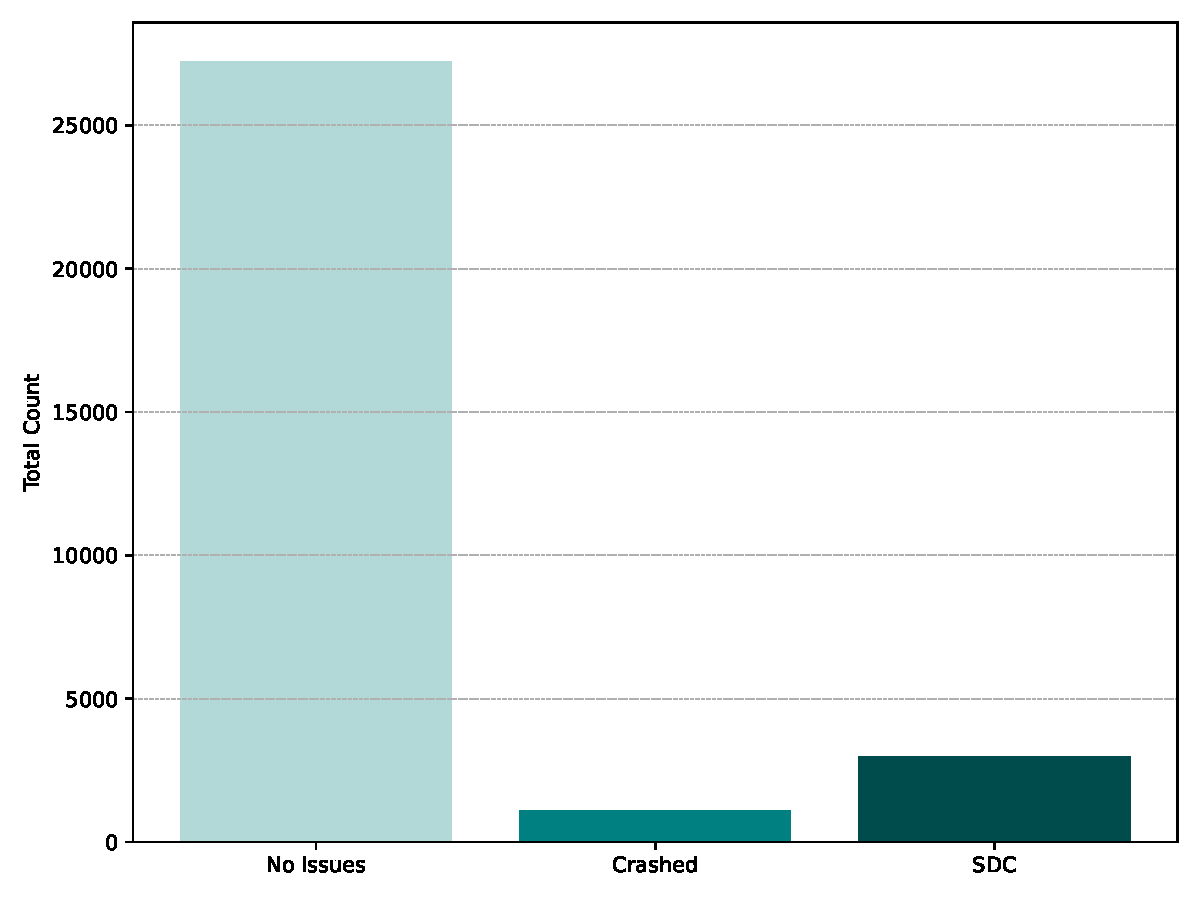
\includegraphics[width=3in]{plots/general_view/general_summary.pdf}
  \caption{Absolute count of observed behavior from all fault injected in first injection campaign.}
  \label{totals}
\end{figure}

Figure \ref{totals} shows us the general results from the first campaign. When looking at the totality of faults injected we clearly see that a vast majority of them do not result in any impact on the normal execution of the program, even when exclusively injecting faults directly into the results of instructions. Only around ten percent of all faults injected had an impact on the final output of the program. Meanwhile an even smaller amount where caught by sanity checks present in the namd benchmark. This result alone already presents a very strong indication that any protection methodology that attempts to protect every single instruction will inevitably spend most its resources catching faults that would not have had an impact on the behavior of the program.\\
%ARREGLAR ALINEAMIENTO
\begin{figure}[!t] 
    \centering
    \subfloat[nab]{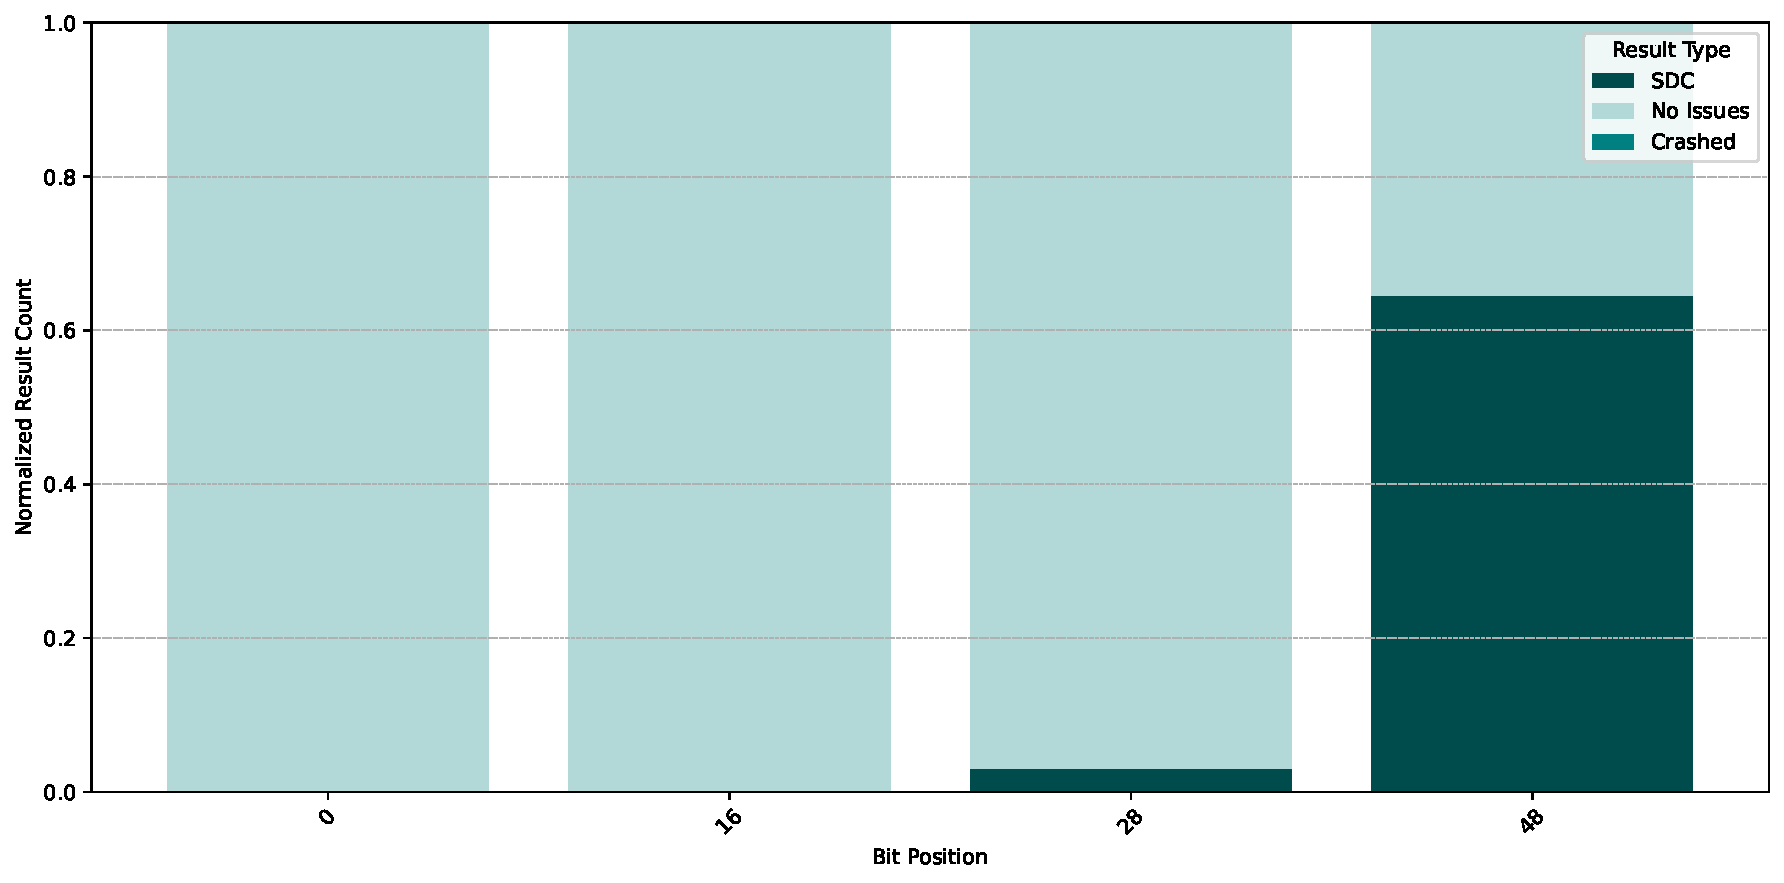
\includegraphics[width=2in]{plots/stacked_distribution/nab_r_stacked_distribution.pdf}}
    \subfloat[namd]{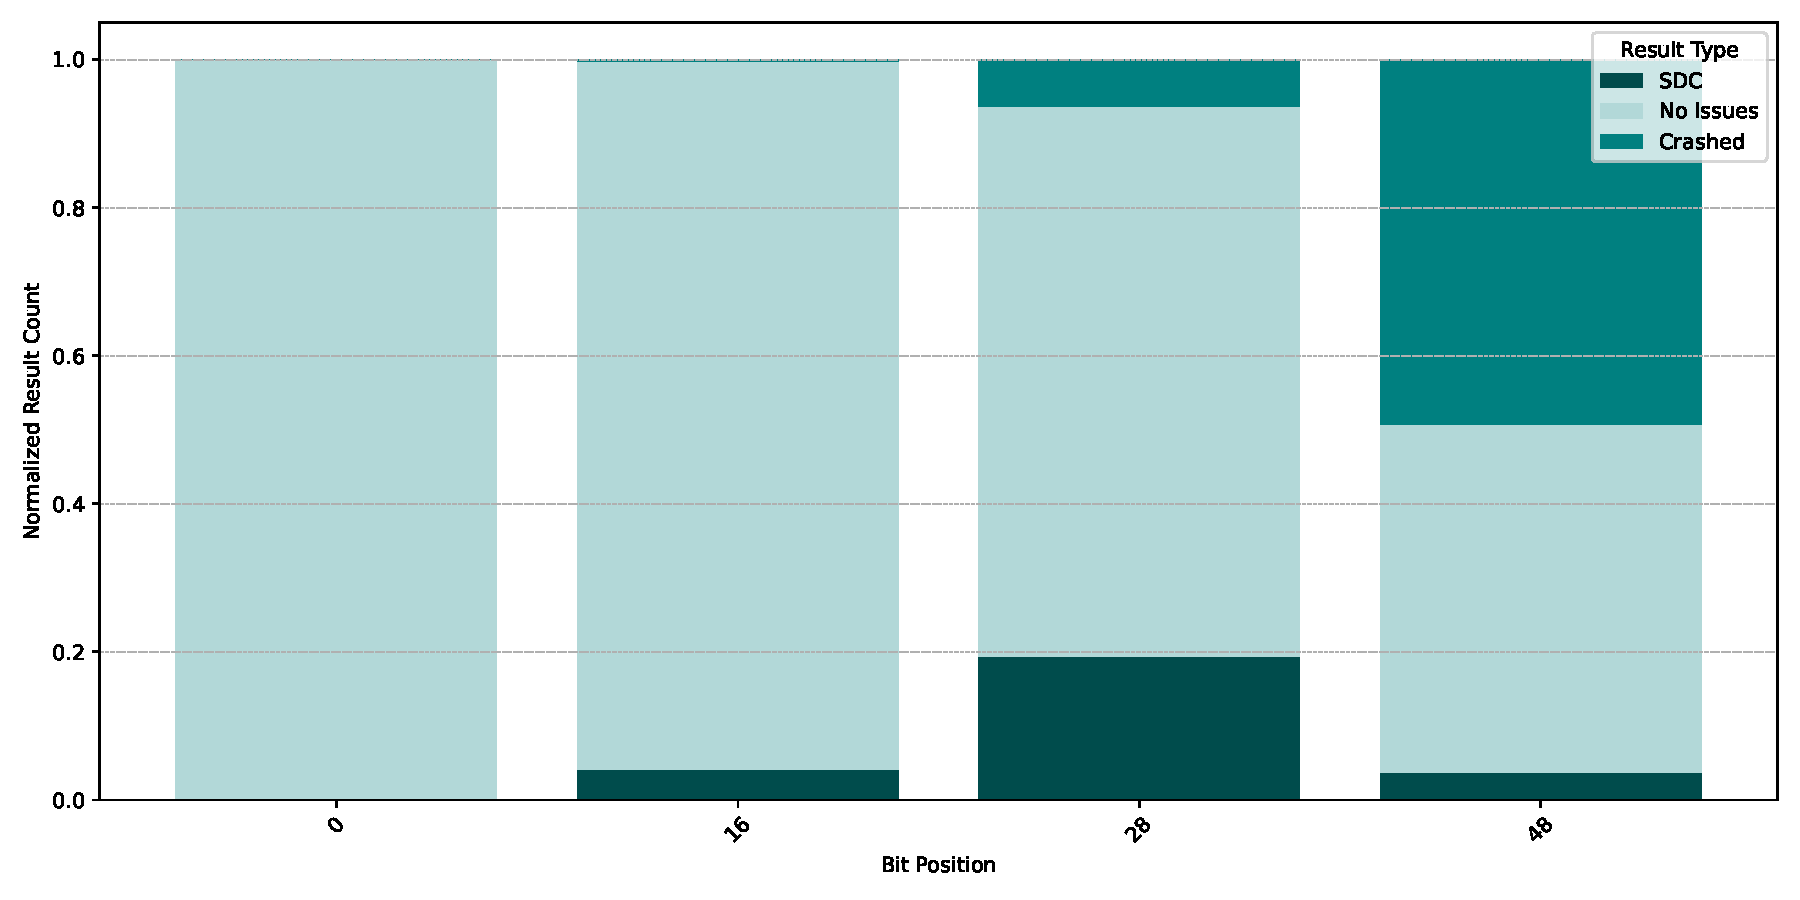
\includegraphics[width=2in]{plots/stacked_distribution/namd_r_stacked_distribution.pdf}}
    \subfloat[wrf]{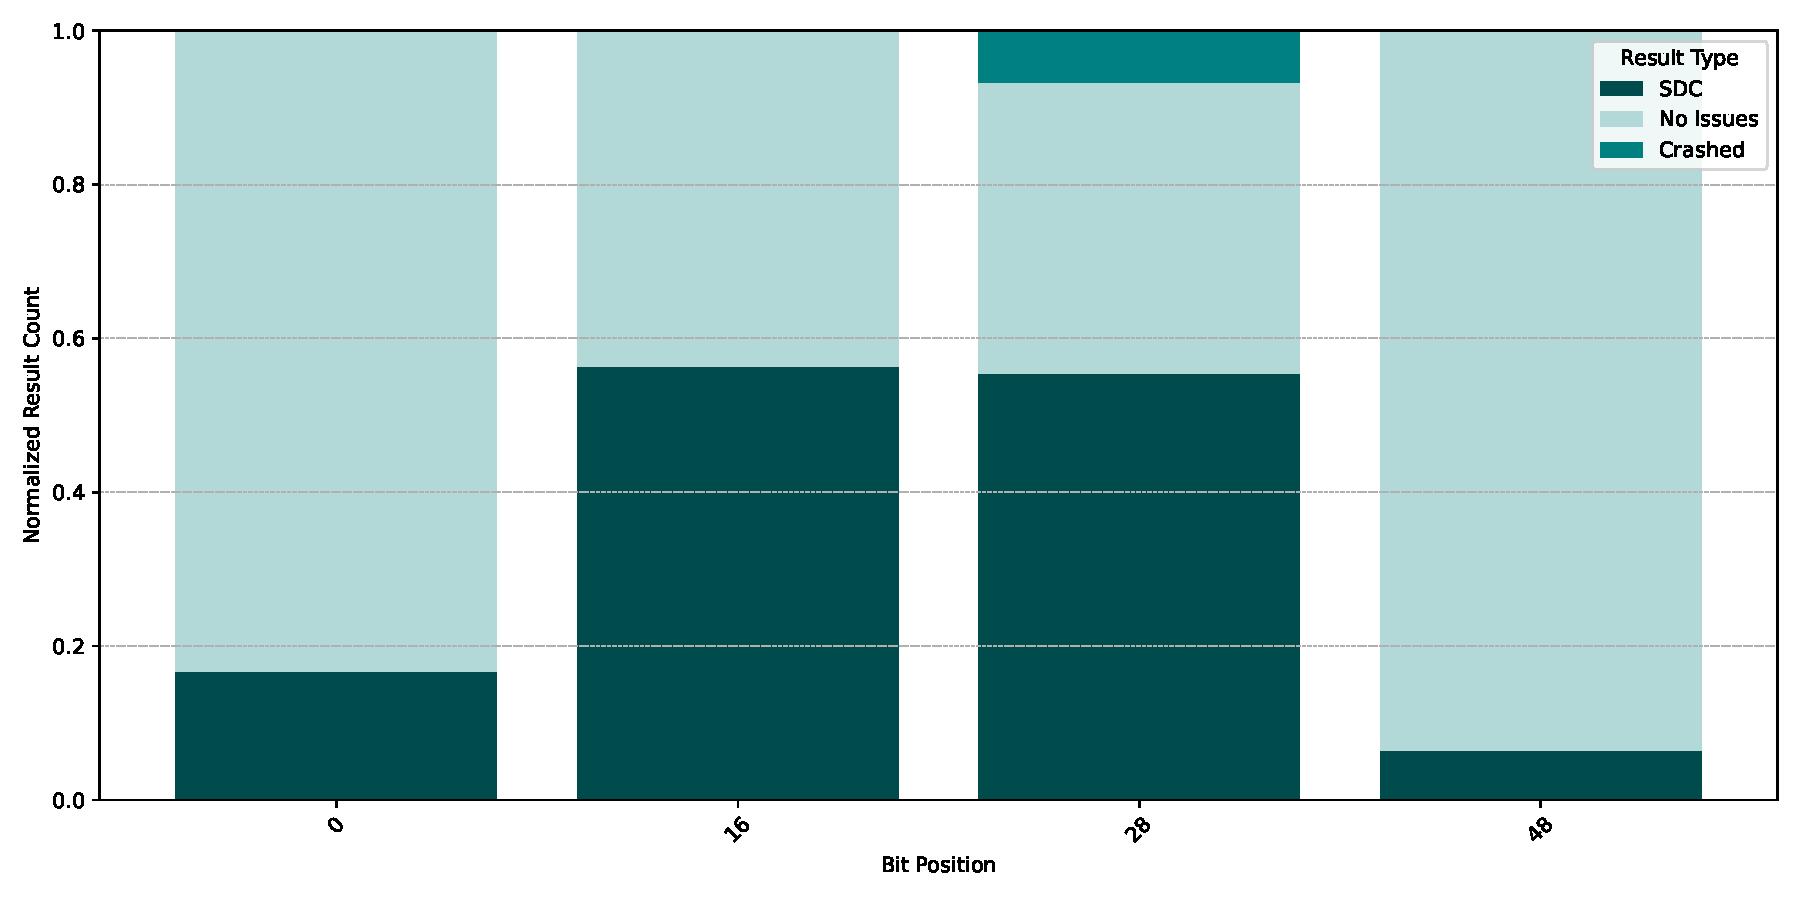
\includegraphics[width=2in]{plots/stacked_distribution/wrf_r_stacked_distribution.pdf}}
\caption{Normalized counts of observed behavior after flipping each respective bit.}
\label{perbits}
\end{figure}

We can go further into the analysis of this first injection campaign. In figure \ref{perbits} we see a breakdown of the results according to the specific bit flipped, here as an example we are showing the plots for the nab and namd benchmarks respectively. With this view some familiar patterns start to emerge. Nab shows the expected behavior one would imagine according to previous literature. As we increase the significance of the bit affected, the amount of runs that result in a visible mismatch in the output increase drastically, observing none on bits 0 and 16, very few at bit 28, and by flipping bit 48 most runs end in an SDC. All other programs instrumented on this campaign showed similar behavior to nab,some showing more sensitivity in the least significant bits, all except wrf and namd. Wrf and namd experience a peak of SDCs in the middle bits, falling of by the most significant. This clashes with the assumed notion that flips in the most significant bits are always the ones that lead to the most SDCs. The specific behavior of every application will be discussed in depth in section  . This plots further give us evidence for the need of granularity if we are to achieve maximum efficiency in protection. Not are faults in most instructions not directly conducive to SDCs, but even inside the result register there are clear differences in priority between bits, which are dependent on the nature of the program currently running. If all bits are protected and if the same strategy is used for all programs, we would be wasting the majority of resources in the protection of non-critical data.\\

Looking further into the data we can separate the observed results groups given by the type of instruction instrumented. Said categories would be ADD, SUB, MUL and DIV instructions. By making this distinction we hoped to see some clear difference in behavior. Having distinctions in criticality between these categories would not only show evidence of our coveted "critical" subsection, but also by being such simple distinctions to make, it would provide evidence that this subsection may be feasible to make out in real time. Figure shows as several things in this regard. First is important to see the clear difference in general sensitivity that different programs carry. Benchmarks likke roms and lbm have SDC rates that at maximum do not exceed ten percent, meanwhile benchmarks like wrf's SDC rates skyrocket to almost 35\% of runs in the case of ADD instructions. This tells us that applications like lbm may benefit from a more lenient protection strategy as it has the certainty that most faults will not end in an error, meanwhile hardware running wrf should have a conservative strategy since any fault that is not caught has a higher chance to result in SDC.\\
\begin{figure}[!t] 
    \centering
    \subfloat[nab]{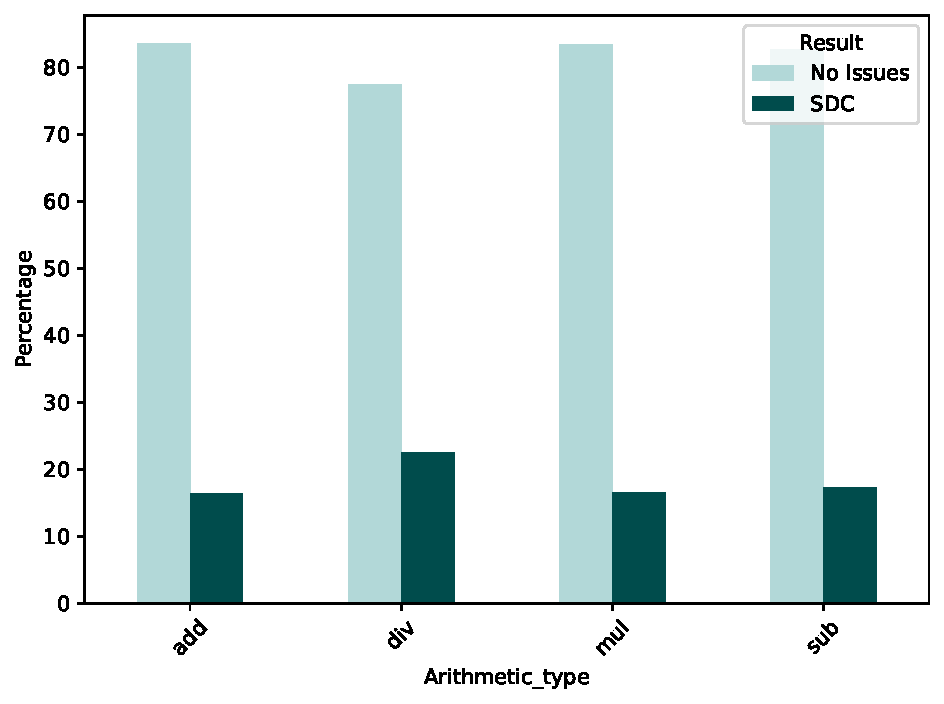
\includegraphics[width=1in]{plots/arithmetic/nab_r_arithmetic_type.pdf}}
    \subfloat[namd]{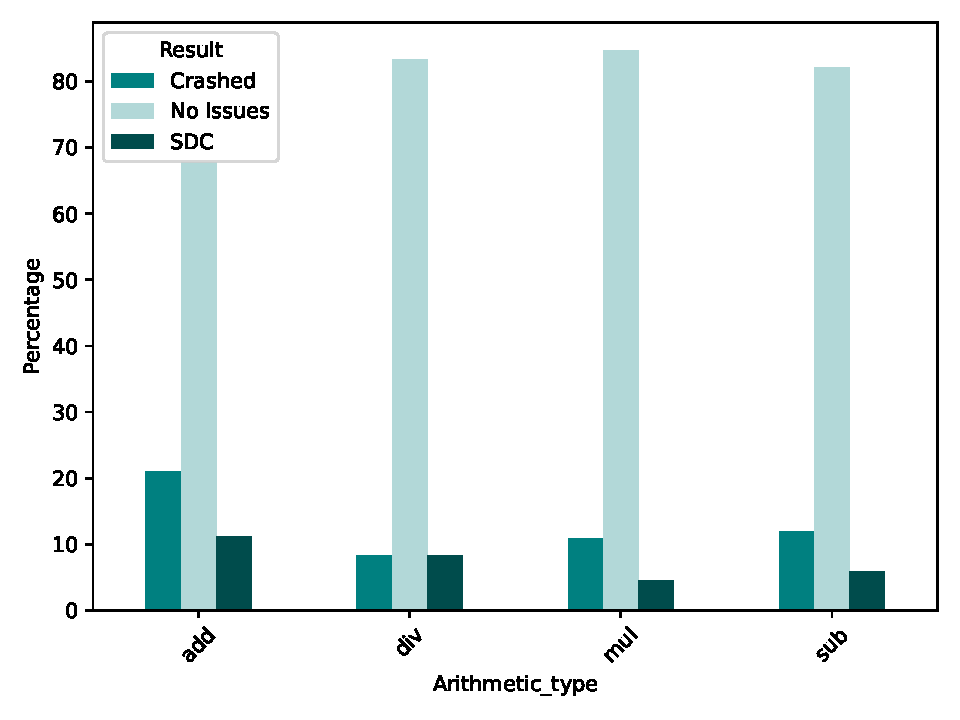
\includegraphics[width=1in]{plots/arithmetic/namd_r_arithmetic_type.pdf}}
    \subfloat[wrf]{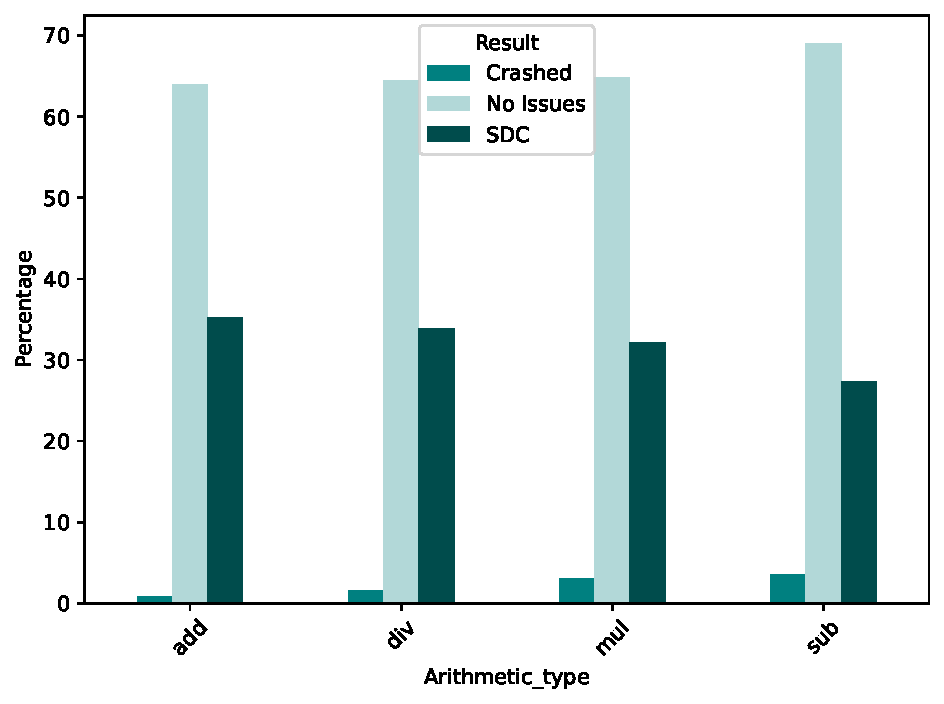
\includegraphics[width=1in]{plots/arithmetic/wrf_r_arithmetic_type.pdf}}
    \subfloat[lbm]{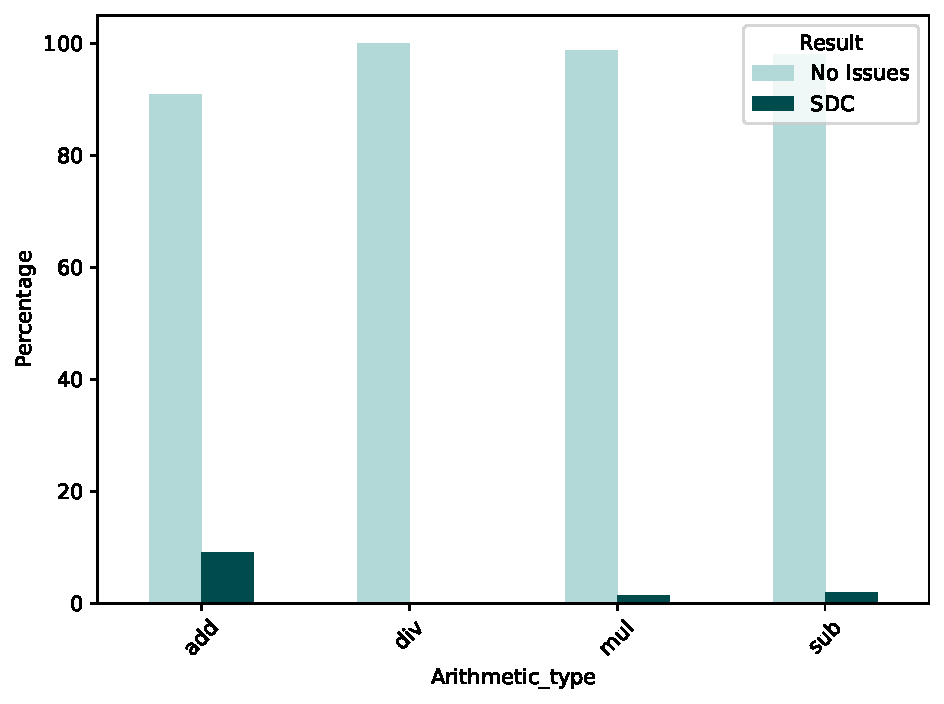
\includegraphics[width=1in]{plots/arithmetic/lbm_r_arithmetic_type.pdf}}
\caption{Normalized counts of observed behavior after flipping each respective bit.}
\label{categories}
\end{figure}
Not only are there differences in the general amount of SDCs, but also we see differences in the distribution of SDCs. Nab has a fairly even distribution between its categories, having a slightly higher sensitivity in DIV instruction. Lbm on the other hand has almost all its SDC coming only from ADD instructions. Already we see a very rough possible candidate for a critical subsection to focus on protection, ADD uinstructions inside lbm, accounting for almost all relevant faults.\\
Spured by this promising reduced experiments, we continued with a more in depth injection campaign on all of SPEC.
\bibliographystyle{IEEEtran}
\bibliography{citations}

\end{document}


